%%%%%%%%%%%%%%%%%%%
% scene

\section{Scény intra}
Intro obsahuje čtyři scény.
Horskou scénu, přímořskou scénu, tunel a jeskyni.
Mezi scénami je plynule přepínáno pomocí zatmívaček.
Zatmívačka je černá plocha.
Tato plocha je kreslena s vypnutým hloubkovým testem.
Ovlivňováním průhlednosti můžeme plynule přejít mezi scénami.
V intru se vyskytují tyto objekty: hory, kopce, skybox, vodní hladina, vodopády, bublinky ve vodě, 
chomáče rostlin, liánové rostliny, bedny, tunel, jeskyně a zavěšené barevné koberce.
\subsection{Horská scéna}
Scéna s horskou scénou je na obrázku \ref{fig:hory}.
Pro vytvoření terénu je použita výšková mapa.
Výšková mapa je vytvořena ze vzdálenostního pole Voroného diagramů, pravá strana ob\-ráz\-ku \ref{fig:voronoid}.
Ve vzdálenostním poli se vyskytují špičky (horské štíty) a propoje (hřebeny).
Na hory je namapována bump mapa, která vytváří skály.
Barva hor je vytvořena dvojicí barevných přechodů.
Jeden barevný přechod je použit stejným způsobem jako na obrázku \ref{fig:gradmap}.
Tímto způsobem získáme barvu s nadmořskou výškou.
Druhý barevný přechod je použit pro obarvení srázů.
Výběr barvy z přechodu je stejný jako u prvního přechodu - pomocí výšky.
Barva je ale přimíchávána pomocí průhlednosti.
Průhlednost je určena podle strmosti srázu - podle normály $n=(u,v,w)$.
Pokud je složka $|v|=1$ je průhlednost maximální.
Při $|v|=0$ je průhlednost minimální.
Kolem hor je skybox, který je zobrazen na obrázku \ref{fig:skybox0}.
S rostoucí vzdáleností se hory noří do mlhy.
Hustota mlhy je vyšší s menší nadmořskou výškou.
\begin{figure}[h]
\centering
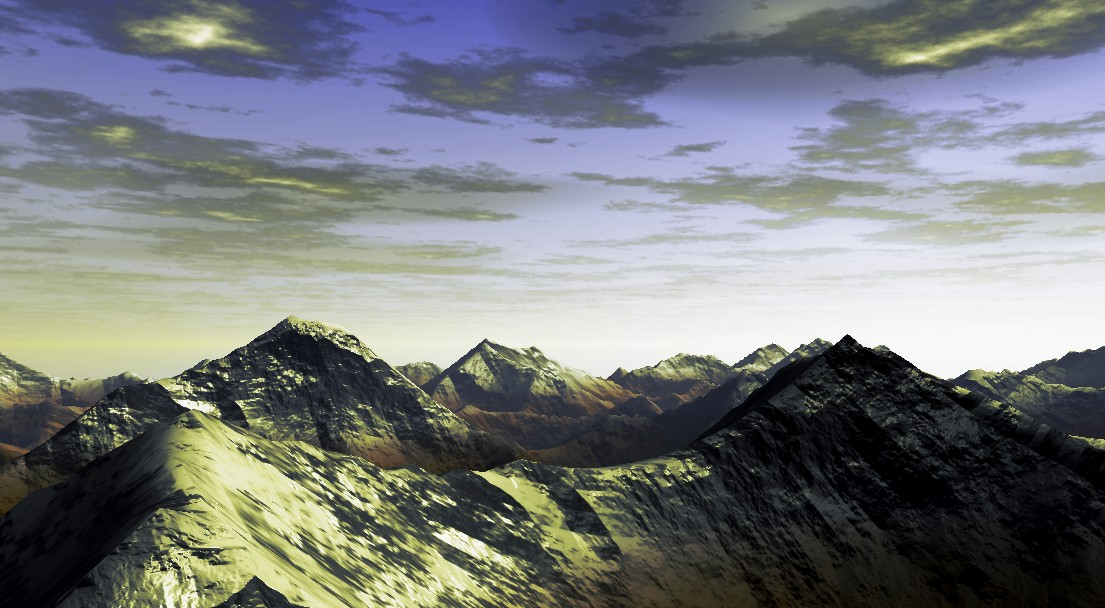
\includegraphics[width=15cm,keepaspectratio]{obr/hory0.jpg}
\caption{Horská scéna.}
\label{fig:hory}
\end{figure}

\subsection{Přímořská scéna}
Přímořská scéna zobrazena na obrázku \ref{fig:pobrezi} je vytvořena pomocí výškové mapy vytvořené ze šumu.
Stejně jako u hor, jsou pro obarvení použity dva barevné přechody.
Skybox kolem přímořské oblasti můžeme vidět na obrázku \ref{fig:skybox1}.
\begin{figure}[h]
\centering
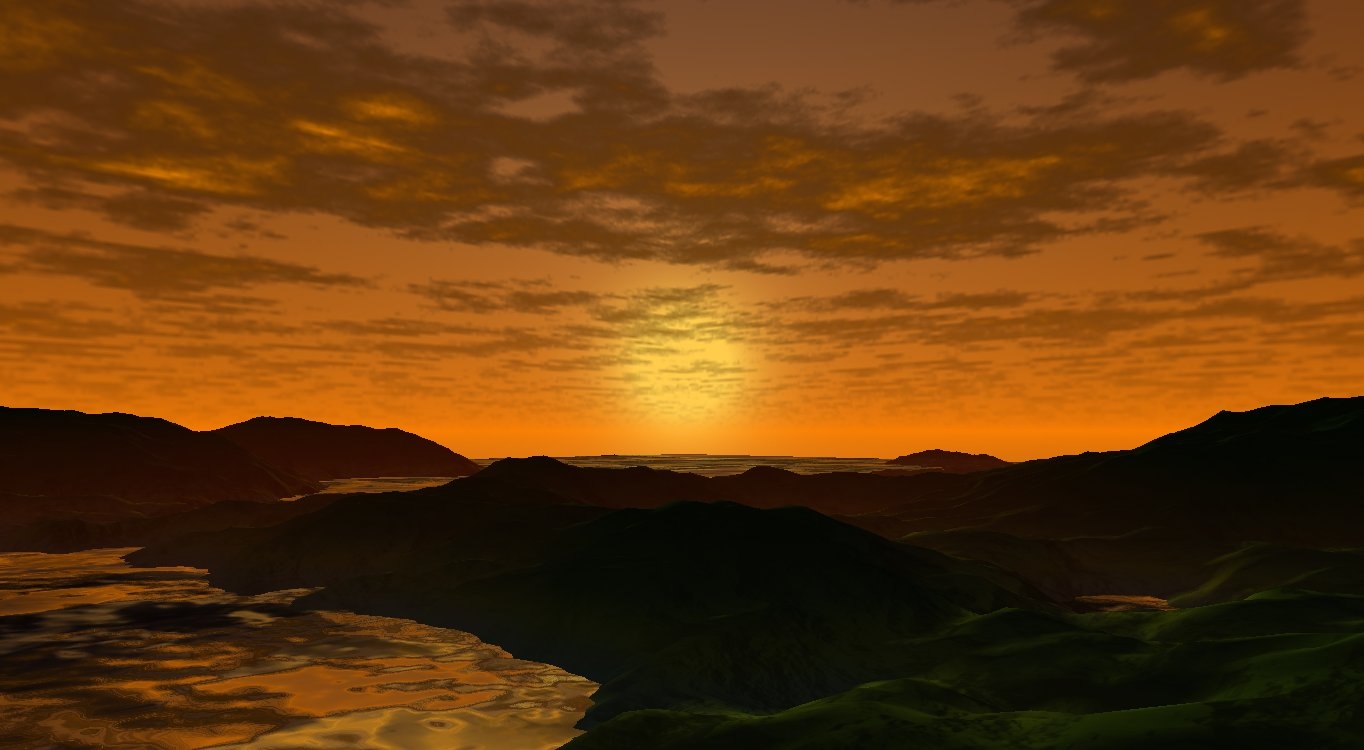
\includegraphics[width=15cm,keepaspectratio]{obr/pobrezi.jpg}
\caption{Přímořská scéna.}
\label{fig:pobrezi}
\end{figure}

\subsection{Tunel, jeskyně}
Tunel i jeskyně jsou vytvořeny stejným způsobem, pomocí algoritmu Marching Tetrahedra.
Rozdíl spočívá ve vytvoření trojrozměrného pole volumetrické reprezentace.
U jeskyně je způsob vytvoření pole jednoduchý.
Vygenerujeme trojrozměrný šum pomocí algoritmu půlení intervalu.
Šum poté vyhladíme pomocí globální transformace.
Poté budeme hodnoty pole násobit koeficientem $k=\langle 0,1 \rangle$.
Hodnota koeficientu $k$ klesá, pokud se vzdalujeme od středu krychle obsahující šum.
Tímto zajistíme, aby se jeskyně uzavřela a neměla ve stěnách díry.
Výslednou objemovou reprezentaci jeskyně převedeme pomocí algoritmu Marching Tetrahedra na trojúhelníky.

Objemová reprezentace tunelu je vytvořena jiným způsobem.
Nejprve vytvoříme troj\-roz\-měr\-ný šum stejně jako u jeskyně.
Hodnoty šumu zmenšíme tak, aby nebyly větší než práh pro algoritmus Marching Tetrahedra.
Pokud bychom teď provedli převod na trojúhelníky, žádný trojúhelník by nevznikl.
Nyní do pole vykreslíme tunel.
Tunel budeme vykreslovat po bodech.
Body leží na křivce podobné jednomu vláknu blesku.
Konce křivky umístíme na opačné rohy krychle šumu.
Křivka je reprezentována dvěma jednorozměrnými šumy.
Jeden ovlivňuje natočení kolem spojnice počátečního a koncového bodu křivky.
Druhý ovlivňuje vzdálenost od spojnice.
Tuto křivku vykreslíme do pole několikrát a vznikne nám tak tunel zobrazený na obrázku \ref{fig:tunel}

Textury v tunelu jsou rozmístěny stejně jako v jeskyni.
Jeskyně je obarvena pomocí několika textur: Textury stropu, textury stěn a textury země.
Každá z těchto textur má k sobě i bump mapu.
Další textura je jednorozměrná a je umístěna vertikálně.
Představuje geologické vrstvy.
Další textura je trojrozměrná.
Je vytvořena pomocí distančního pole z Voroného diagramů a reprezentuje kaustiky.
Textura je trojrozměrná, abychom mohli kaustiky animovat.
Poslední textura je také trojrozměrná a je dynamicky měněna.
Před\-sta\-vu\-je vlhkost stěn jeskyně.
Vodopády do ní zapisují hodnoty a textura samotná ovlivňuje míru odlesků a tmavost povrchu.

V tunelu jsou umístěny chomáče rostlin.
Jedná se o částicový systém, jehož částice jsou statické.
Textura částic je zobrazena v levé části obrázku \ref{fig:listy}.
Na konci tunelu je vodní hladina.
V tunelu se vyskytuje i pavučina.
Pavučina je složena z elastického systému	a můžeme ji vidět uprostřed obrázku \ref{fig:tunel}.

V jeskyni jsou zavěšeny liánové rosliny.
Rostliny jsou složeny z elastického systému, jehož tvar je v pravé části obrázku \ref{fig:listy}.
Jeden článek rostliny je složen ze dvou spojených čtyřstěnů.
V bodech je umístěna textura rosliny zobrazena v levé části obrázku \ref{fig:listy}.
Dalším objektem jeskyně je zavěšený koberec.
Koberec je také složen z elastického systému ve tvaru mřížky.
Na koberec je nanesena textura na obrázku \ref{fig:koberec}

\begin{figure}[h]
\centering
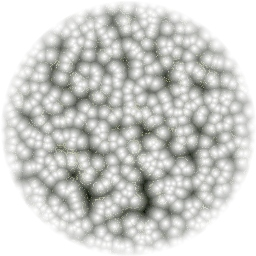
\includegraphics[width=3cm,keepaspectratio]{obr/listy.jpg}
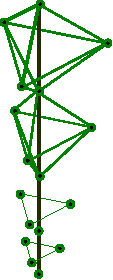
\includegraphics[width=2cm,keepaspectratio]{obr/liana.pdf}
\caption{Vlevo: textura rostlin.
Vpravo: rozložení uzlů a spojů elastického systému liánové rostliny.}
\label{fig:listy}
\end{figure}

\begin{figure}[h]
\centering
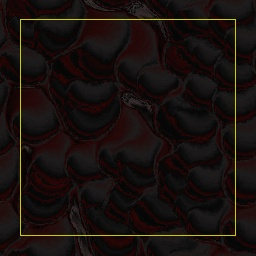
\includegraphics[width=4cm,keepaspectratio]{obr/koberec.jpg}
\caption{Textura zavěšeného koberce.}
\label{fig:koberec}
\end{figure}

\begin{figure}[h]
\centering
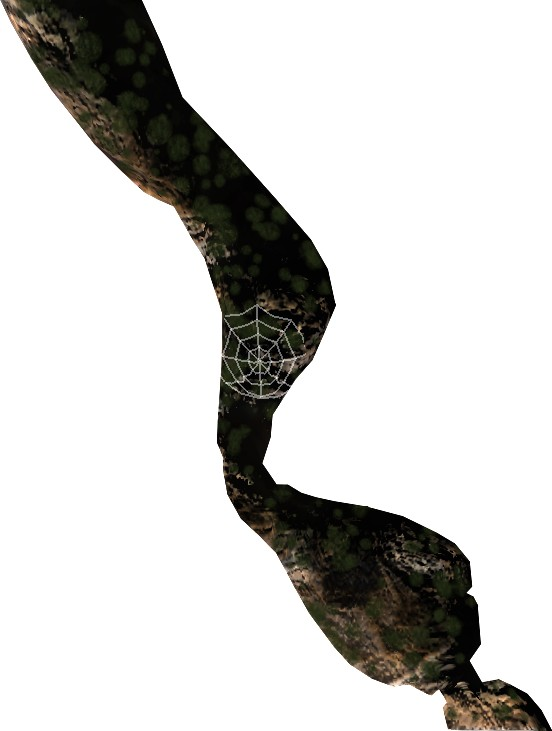
\includegraphics[width=7.5cm,keepaspectratio]{obr/tunel.jpg}
\caption{Tunel.}
\label{fig:tunel}
\end{figure}

\begin{figure}[h]
\centering
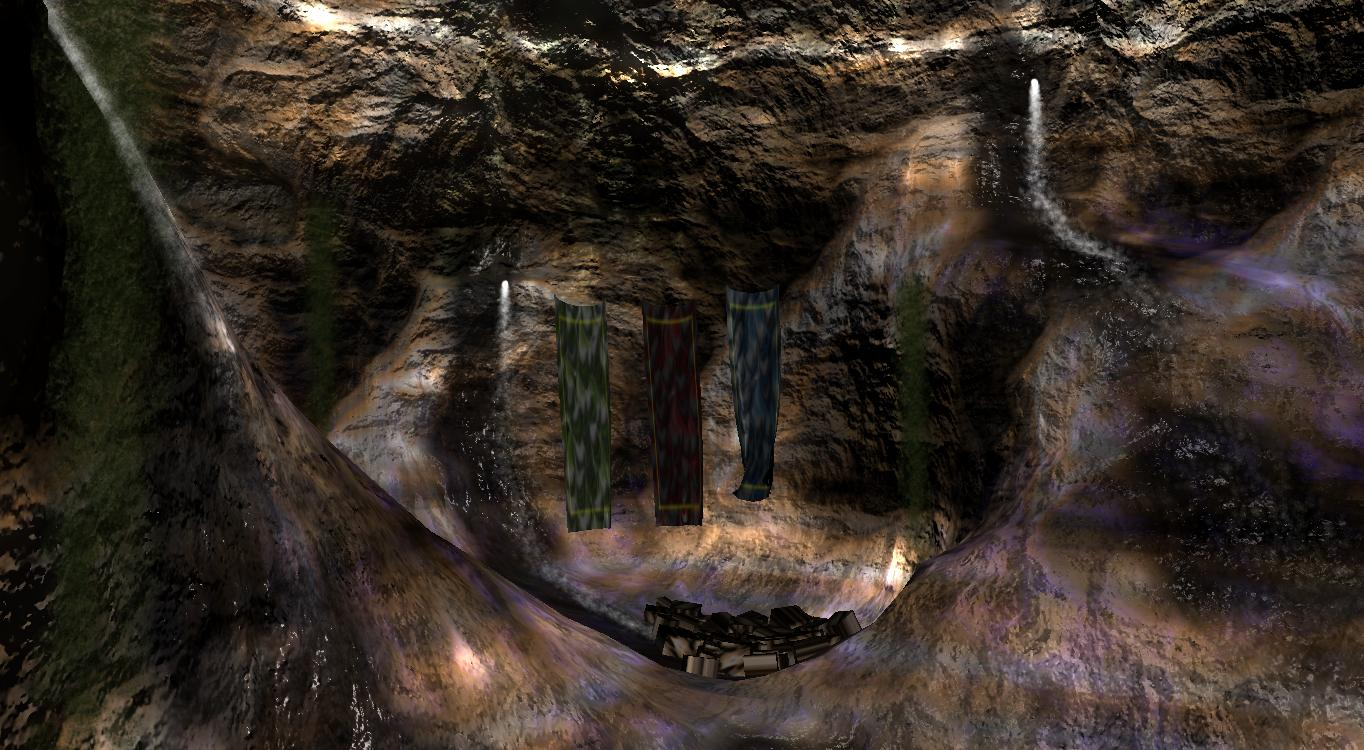
\includegraphics[width=15cm,keepaspectratio]{obr/jeskyne.jpg}
\caption{Jeskyně.}
\label{fig:jeskyne}
\end{figure}






